% !TEX encoding = UTF-8 Unicode

% Beispiel für ein LaTeX-Dokument im Format "seminarvorlage"
\documentclass[ngerman]{seminarvorlage}
% ngerman = Deutsch in neuer Rechtschreibung, alternativ english
\usepackage[utf8]{inputenc} % Kodierung der Umlaute
\usepackage{babel} % automatische Sprachanpassung, Sprache siehe oben
\usepackage{cleveref} % für bequeme Referenzen, siehe \cref unten

%Own Code
\usepackage{needspace}	
\usepackage{amsmath}
\usepackage{listings}
\usepackage{xcolor}
\lstset { %
    language=C++,
		commentstyle=\color{gray},
    backgroundcolor= \color{black!4}, % set backgroundcolor
    basicstyle= \small,%\tiny,%\footnotesize,% basic font setting
		showtabs=false,
		tabsize=1,
		breaklines=true,
		numbers=left,
		 showspaces=false,
		showtabs=false,
		keepspaces=true,
				 numbersep=1pt,
  showstringspaces=false,
	aboveskip=5pt,
belowskip= -10pt
}

\newcommand*{\fullref}[1]{\hyperref[{#1}]{\autoref*{#1} \nameref*{#1}}} % One single link
\newcommand*{\quelle}{% 
  \footnotesize Quelle: 
} 

\begin{document}
% Unbedingt angeben: Titel, Autoren, E-Mail
% Freiwillig: Adresse
\title{Embedded Realtime OS FreeRTOS auf STM32F4}
\numberofauthors{2}
\author{
  \alignauthor Michael Ebert\\
		\affaddr{Ad-hoc Networks GmbH}\\
    \email{ebert@ad-hoc.network}
  \alignauthor Christoph Bläßer\\
		\affaddr{Bundesamt für Sicherheit in der Informationstechnik}
    \email{christoph.blaesser@gmx.de}
}

\maketitle
\keywords{ FreeRTOS, RTOS, ARM , STM32, Real Time.}
\abstract{
Im Rahmen dieser Arbeit wird das Echtzeitbetriebssystem FreeRTOS vorgestellt. Hierzu werden zu Beginn die allgemeinen Eigenschaften für Echtzeitbetriebssysteme beschrieben. Im Verlauf des Textes wird an ausgewählten Beispielen dargestellt, wie FreeRTOS diese Anforderungen berücksichtigt und durch geeignete Programmfunktionen umsetzt.
}
\section{Grundlagen Echtzeitsysteme}
%!TEX root = FreeRtos ARM uController.tex


\subsection{Echtzeitsysteme und Echtzeitbetriebssysteme}
\label{sec:Echtzeitsysteme}
Mit der steigenden Leis\-tungs\-fähig\-keit von modernen $\mu$\-Pro\-zesso\-ren, steigen auch die Anforderungen an die Software die auf diese Systeme aufsetzt. Viele dieser Systeme fordern trotz ihrer Komplexität, dass Teile des Pro\-gramm\-ab\-laufs in bestimmten zeitlichen Grenzen ausgeführt werden und somit vorhersehbar und deterministisch sind. Systeme die solchen Anforderungen unterliegen werden Echtzeitsysteme genannt. Bezogen auf ihre Zuverlässigkeit unterliegen Echtzeitsysteme einer weiteren Unterteilung, in Echtzeitsysteme mit weicher Echtzeitanforderung (soft realtime systems) und Echtzeitsysteme mit harter Echtzeitanforderung (hard realtime systems). Ein weiches Echtzeitsystem soll eine Aufgabe in den vorgegebenen zeitlichen Grenzen ausführen. Ein Über\-schreiten der zeitlichen Grenzen ist grundsätzlich nicht erlaubt, führt aber nicht unmittelbar zu einem Fehler oder einem Versagen des Gesamtsystems. Ein hartes Echtzeitsystem hingegen muss die gestellte Aufgabe in den vorgegebenen Grenzen aus\-füh\-ren. Durch eine Überschreitung wird das System unbrauchbar und führt dazu, dass das System nicht im vorgesehenen Szenario eingesetzt werden kann. Dabei ist ausdrücklich zu beachten, dass Echtzeit nicht bedeutet, dass ein Programm besonders schnell ausgeführt wird. Die Ausführung eines Programms kann beispielsweise auch gewollt langsam sein und gerade deshalb den gestellten Echtzeitanforderung genügen. Einige Beispielsysteme und deren Echtzeitzuordnung wird in Tabelle \ref{tab:BeispieleEchtzeitsystem} gezeigt. 
\begin{table*}
\centering
	\begin{tabular}{|l|l|l|}
		\hline
		\textbf{Beispiel} & \textbf{Echtzeit Typ}  & \textbf{Auswirkung} \\
		\hline
		Tastatur Controller & Soft Realtime & Kurzfristig verzögerte Ausgabe \\
		\hline
		Echtzeit Media Streaming  & Soft Realtime & Bild und Ton kurzfristig asynchron \\
		\hline
		Computer Numerical Control (CNC)  & Hard Realtime & Fehler bei der Fertigung des Teils\\
		\hline
		Airbag System  & Hard Realtime & Möglicher Personenschaden\\
		\hline
	\end{tabular}
	\caption{Beispiele von Echtzeitsystemen und deren Auswirkung beim über- oder unterschreiten der Anforderungsgrenzen}
	\label{tab:BeispieleEchtzeitsystem}
\end{table*}
Um die grund\-sätz\-liche Funktionalität eines Echtzeitbetriebssystems zu erläutern, werden zuerst die Grundmodelle für den Programmablauf eingebetteter Systeme beschrieben. Der Programmablauf lässt sich auf drei Modelle zu\-rück\-füh\-ren (Abbildung \ref{fig:Programmablauf}). 
\begin{figure}[ht]
	\centering
		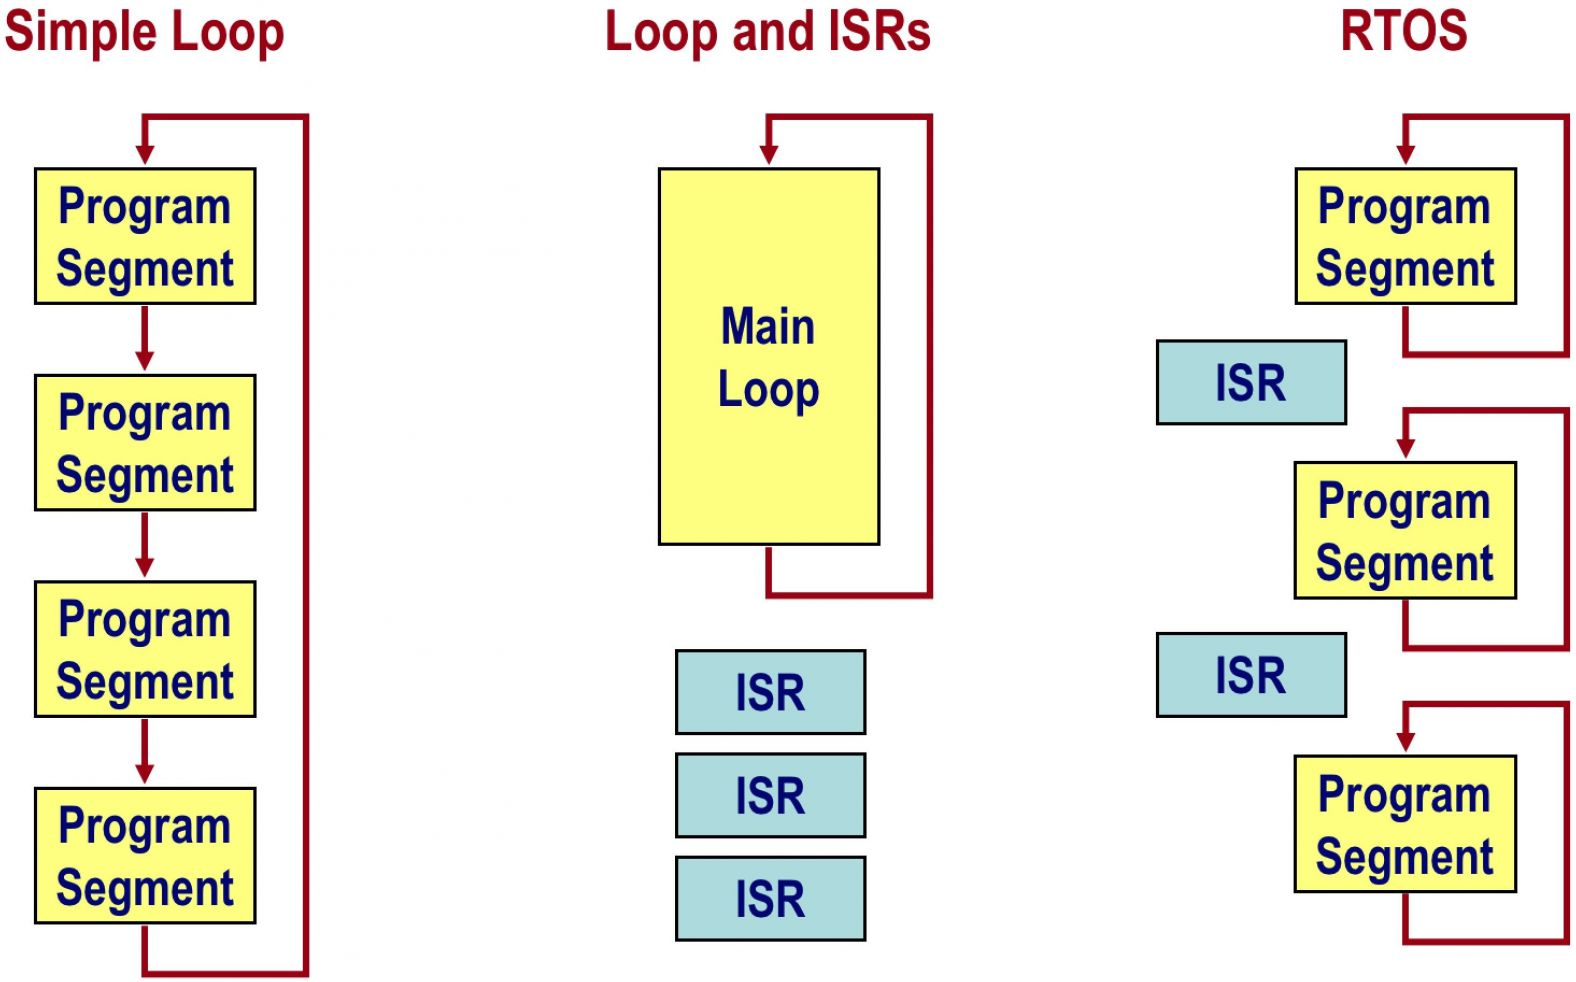
\includegraphics[width=0.3\textwidth]{Pictures/EmbeddedCom/cwrtos2f5c.jpg}
	\caption{Übersicht Programmabläufe in embedded Anwendungen. Unterscheidung von zwei Hauptkategorien: Schleifen-gesteurte Anwendungen und Event-gesteurte Anwendungen. Bild-Quelle~\protect\citeA{RTOSRevealed}}
	\label{fig:Programmablauf}
\end{figure}
Eingebettete Anwendungen können in einer einzigen Schleife (mit oder ohne Interrupt Unterbrechungen) laufen oder aber in event-gesteuerten ne\-ben\-läuf\-igen ei\-gen\-stän\-dig\-en Pro\-gramm\-ab\-schnit\-ten (Thre\-ad oder Task\footnote{Nachfolgenden wird Task benutzt, da dies der geläufige Begriff bei FreeRTOS ist. In der Literatur zu Echtzeitsystemen ist der Begriff nicht exakt definiert.}) ausgeführt werden. Die ne\-ben\-läuf\-ige Aus\-füh\-rung der unterschiedlichen Programmsegmente ist nur durch einen Scheduler, welcher Teil eines RTOS Kernels ist, zu erreichen. Ein RTOS Kernel abstrahiert von der zugrunde liegenden Hardware und ermöglicht weitergehende Steuerung, beispielsweise durch Verwaltung von Timing Informationen. Der Kernel stellt durch den Scheduler sicher, dass die näch\-ste Task rechtzeitig ausgeführt wird. Der Entwickler ist dafür verantwortlich, dass die Task die ge\-wün\-schte Aufgabe im zeitlichen Rahmen ausführt. Durch den Einsatz des RTOS Kernels kann der Entwickler jedoch auf Spezifika der Hardware verzichten und die Funktionen des Kernels verwenden. Wie sichergestellt werden kann, dass eine Task harten oder weichen Echtzeitanforderungen entspricht, wird Abschnitt \ref{sec:Echtzeitanalyse} beschrieben. Für viele kleine Anwendungen kann die Nutzung einer einzigen Schleife durchaus sinnvoll sein, wenn beispielsweise die Ressourcen so knapp sind, dass ein Overhead durch zusätzliche Verwaltungsfunktionen ausgeschlossen werden muss. Ein großer Nachteil der "`einschleifen Variante"' ist die permanente Nutzung des Prozessors, auch "`processor hogging"' oder "`CPU hogging"' genannt. Um den Prozessor in dieser Variante in einen Energiesparmodus zu versetzen sind umfangreiche Kenntnisse über den Prozessor sowie eine sehr strukturierte Programmierung erforderlich, die gerade bei Anpassungen der Software zu Problemen führen kann. Besonders bei akkubetriebenen Geräten wie IoT Devices oder Mobiltelefonen wird sehr genau auf die Energieaufnahme geachtet. Ein RTOS Kernels hingegen arbeiten mit einem Event gesteuerten Programmablauf, ein "`CPU hogging"' kann somit vermieden werden. Des Weiteren bieten viele RTOS Kernel sehr einfache Lösungen zur effektiven Nutzung von Energiesparmodis. Dies wird in Abschnitt \ref{sec:Low Power Modes} am Beispiel von FreeRTOS und einem ARM $\mu$Prozessor demonstriert. Neben der Echt\-zeit\-fähig\-keit gibt es aber noch viele weitere Vorzüge für den Einsatz eines Echtzeitbetriebssystems. Durch das Herunterbrechen der Anwendungen in Tasks entstehen viele kleine Module, die jeweils eine kleine Teilaufgabe des Gesamtsystems über\-neh\-men. Durch ein sauber definiertes Interface zur Kommunikation der Tasks, lässt sich die Entwicklungsarbeit leicht auf mehrere Teams verteilen. Dies ermöglicht auch den Einsatz von agilen Entwicklungsmethoden wie Scrum in der Entwicklung von eingebetteten Systemen. Ein weiterer großer Vorteil ist die Erweiterbarkeit von RTOS Anwendungen. Bei Änderungen von Anwendungen die in einer Schleife laufen, ist oft der gesamte Code von dieser Änderungen betroffen. Ein RTOS hat durch die Interprozesskommunikation eine natürliche Lose-Kopplung zwischen den einzelnen Programmfunktionalitäten. Das Än\-dern oder Hinzufügen von Tasks ist somit wesentlich einfacher, da andere Tasks nicht unmittelbar durch diese Än\-der\-ung betroffen sind. 




 
\section{FreeRTOS} 
%!TEX root = FreeRtos ARM uController.tex
\subsection{Geschichte}
FreeRTOS wird seit etwa 10 Jahren von der Firma Real Time Engineers Ltd. in Zusammenarbeit mit verschiedenen Chipherstellern entwickelt. Derzeit unterstützt es 35 Architekturen und wurde mehr als 113000 mal heruntergeladen. Das Entwicklerteam unter Führung des Gründers Richard Barry konzentrieren sich bei der Entwicklung darauf sowohl ein geeignetes Qualitätsmanagement umzusetzen, als auch die Verfügbarkeit der verschiedenen Dateiversionen zu gewährleisten. FreeRTOS wird in zwei verschiedenen Lizenzmodellen angeboten, die eine Anpassung der originären GNU General Public Licence darstellen. Die Open Source Lizenz (FreeRTOS) erhält keine Garantien und keinen direkten Support. Entwickler die diese freie Lizenz verwenden und Än\-der\-ungen am RTOS Kernel vornehmen, müssen den Quellcode ihrer Än\-der\-ungen für die Community offenlegen. In der kommerziellen Lizenz (SafeRTOS) können solche Änderungen als closed source vertrieben werden. Kunden mit einer kommerziellen Lizenz bietet Real Time Engineers Ltd. Unterstützung bei der Entwicklung von Projekten und Treibern. Des Weiteren werden entsprechende Garantie für die Echt\-zeit\-fähig\-keit von SafeRTOS gegeben. Real Time Engineers bietet zu FreeRTOS diverse Erweiterungen wie Treiber und Tools. Geführt werden diese Erweiterungen unter dem Namen FreeRTOS Ecosystem, dazu gehören unter anderem ein FAT Dateisystem, TCP/ UDP Stacks, sowie TLS/SSL Implementierungen. 
%!TEX root = FreeRtos ARM uController.tex
\subsection{Entwicklungsumgebung}
FreeRTOS ist im Prinzip nicht an eine spezielle Entwicklungsumgebung gebunden. Dies liegt vor allem daran, dass FreeRTOS in Form von C-Quellcodedateien zur Verfügung gestellt wird und alt Teilkomponente mit in die zu entwickelnde Software integriert wird. Die verwendete Entwicklungsumgebung muss lediglich einen geeigneten Compiler zur Verfügung stellen. Vor dem Start eines Entwicklungsprojektes ist es dennoch ratsam sich einen Überblick über die ver\-fügbaren IDEs\footnote{Integrated Development Environment} zu machen. Der wichtigste Punkt der hierbei zu berücksichtigen ist, ist das Debugging. Da ein Echtzeitbetriebssystem eine weitere Abstraktionsebene hinzufügt und wie eine Art Middleware fungiert, lassen sich viele RTOS spezifische Funktionen und Eigenschaften wie Queues, Task Stacks etc. nur mühsam mit einem Debugger wie GDB untersuchen. Viele der marktgängigen Entwicklungsumgebungen bieten daher spezielle RTOS-aware Pakete, so dass ein einfacherer Zugriff auf RTOS Objekte und Eigenschaften möglich ist. Wie die RTOS awareness beim Debugging eingesetzt wird und welche Funktionalitäten sie einem Entwickler bietet wird in Abschnitt \ref{sec:Debugging von Echtzeitsystemen} aufgezeigt. Ein weiterer Punkt der bei der Auswahl der IDE betrachtet werden muss sind die Kosten. Bei proprietären IDEs können oft mehrere tausend Euro Lizenzkosten anfallen. Diese bieten aber den Vorteil der nahtlosen Einbindungen von $\mu$Prozessoren und Echtzeitbetriebssystemen (RTOS awareness). Bei der Entwicklung von ARM $\mu$\-Prozessoren sind hier Keil (Arm), IAR Workbench und True Studio (Atollic) zu nennen. Diese Entwicklungsumgebungen lassen sich zum Teil auch frei verwenden, allerdings mit starken Einschränkungen wie z.B. der maximalen Codelänge. Auf der nicht proprietären Seiten steht Eclipse CDT. Es ist komplett frei in der Verwendung und hat keine Beschränkungen. Der Nachteil ist hier, dass die Integration nicht so einfach ist, wie bei den proprietären IDEs. RTOS awarness wird bei Eclipse durch die Installation weiterer Plugins erreicht. Ein weiterer Nachteil sind die fehlenden Beispielprojekte für Eclipse CDT in der Kombination mit FreeRTOS. Daher müssen Projekte von Grund auf selbst konfiguriert und installiert werden. Da im Laufe dieser Arbeit Eclipse CDT für alle Beispiele verwendet wird, wird in Abschnitt \ref{sec:Einrichtung und Konfiguration} das Aufsetzen einer Basiskonfiguration erklärt. 

%!TEX root = FreeRtos ARM uController.tex
\subsection{Zielsysteme STM32F4 (ARM Cortex M4)}
Der STM32F4 ist ein von STMicroelectronics entwickelter 32 Bit uController basierend auf einem ARM Cortex M4 Kern. Der STM32F4 läuft auf maximal 168 Mhz. Neben seinen unzähligen Schnittstellen (4x UART, SPI, I2C, Ethernet) bietet der STM32F4 mehrere Energiespar-Modis, die ihn für den Einsatz in energieeffiziente Anwendung, wie IOT Devices interessant machen. Für die Verwendung von FreeRTOS eignet sich der uController besonders gut, da speziell für diesen uController viele Hardware-Funk\-tio\-na\-li\-tät\-en in den FreeRTOS Kernel integriert wurden. Der STM32F4 ist seit 2012 auf dem Markt und erfährt durch eine große Anzahl an online Beispielen eine hohe Beliebtheit in der Entwickler Community. Zum Zugriff auf uController Funktionen stellt STM das Hardware Abstraction Layer, kurz HAL zur Verfügung, sie Abbildung \ref{fig:HAL}.      
\begin{figure}[htb!]
	\centering
		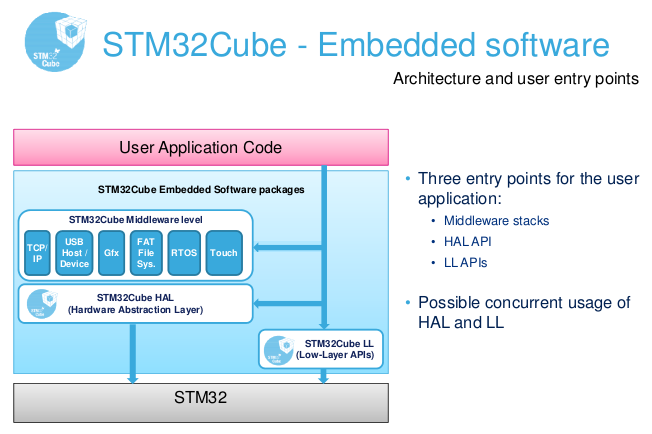
\includegraphics[width=0.4\textwidth]{Pictures/STM32F4/LibraryEntry.png}
	\caption{Aufbau der zur Verfügung stehenden STM Bibliotheken }
	\label{fig:HAL}
\end{figure}
\newline
Die HAL ermöglicht eine einfache Verwendung der Hardware ohne großen Konfigurationsaufwand. Wie spezielle Hardware-Funktionen des STM32F4 durch FreeRTOS genutzt werden, wird in Abschnitt \ref{sec:Low Power Modes} und Abschnitt \ref{sec:Memory Protection} gezeigt.
%!TEX root = FreeRtos ARM uController.tex
\subsection{Einrichten und Konfiguration}
\label{sec:Einrichtung und Konfiguration}
Dieser Abschnitt beschreibt die Einrichtung eines FreeRTOS Projektes für den STM32F4. Die Beschreibung dabei ist nicht vollständig und versteht sich eher als eine Art Leitfaden. Alle anwendungsspezifischen Konfigurationen können in den zur Verfügung gestellten Links nachgelesen werden. Hierbei ist besonders die Seite des GNU ARM Plugins hervorzuheben, da diese einen guten Einstieg für die Erstellung eines ARM Projekts bietet. Als Entwicklungsumgebung wird Eclipse CDT verwendet, welches bereits in Abschnitt \ref{ref:Entwicklungsumgebung} beschrieben wurde. Als Host System wird hier Windows verwendet, die Einrichtung unter Linux ist aber ähnlich.Nach der Installation von Eclipse muss das GNU ARM Plugin für Eclipse CDT installiert werden. Dieses ist entweder über den Pluginmanager oder über den folgenden Link erhältlich: 
\newline
\newline
http://gnuarmeclipse.github.io/
\newline
\newline
Das Plugin ermöglicht die Einbindung und die Konfiguration von ARM Cross Compilern. Des Weiteren stellt es einige Beispielprojekte für ARM $\mu$Controller zur Verfügung. Nach der Installation des ARM Plugins, müssen die GCC ARM Toolchain und die GNU Build Tools installiert werden. 
Diese können unter den folgenden Webadressen heruntergeladen werden: 
\newline
\newline
https://launchpad.net/gcc-arm-embedded
\newline
https://github.com/gnuarmeclipse/windows-build-tools/
\newline
\newline
Die Toolchain und die Buildtools stellen Anwendungen bereit, die zum Kompilieren und Debuggen der C und C++ Dateien benötigt werden. Zur Toolchain gehören unter anderem GCC als Cross Compiler und GDB (GNU Debugger) zum Debuggen der Anwendung auf der Zielplattform. Die GNU Buildtools beinhalten make und rm, die zum Organisieren des Builds benötigt werden. Nach der Installation müssen die Verzeichnisse der Toolchain und der Buildtools im Plugin konfiguriert werden. Mit dieser Konfiguration ist das System nun in der Lage C und C++ Dateien für die Zielplattform zu kompilieren und als Binary File (.elf) bereitzustellen. Zum Übertragen und Debuggen der Anwendung auf dem Zielsystem wird ein ISP-Programmer für ARM benötigt.\needspace{5\baselineskip} Folgende ISP-Programmer werden häufig verwendet, dabei ist Liste weder vollständig, noch stellt sie eine Empfehlung dar.
\begin{itemize}
	\item Segger J-Link:
	\newline
	https://www.segger.com/jlink-debug-probes.html
	\item Keil Ulink: 
	\newline
	http://www2.keil.com/mdk5/ulink
	\item STM ST-Link/VL: 
	\newline
	http://www.st.com/en/development-tools/st-link-v2.html
\end{itemize}
Zur Nutzung des ISP müssen die benötigten Treiber und der On-Chip Debugger des Herstellers installiert werden. Eine Alternative zum On-Chip Debugger des Herstellers ist OpenOCD. Details dazu findet man unter:
\newline
\newline
http://openocd.org/
\newline
\newline            
Nachdem die Konfiguration der Entwicklungstools abgeschlossen ist, kann nun ein Basis Projekt erstellt werden. Hierfür empfiehlt sich ein Templateprojekt des GNU ARM Plugins, siehe Abbildung \ref{fig:NewProj}.
\begin{figure}[htb]
	\centering
		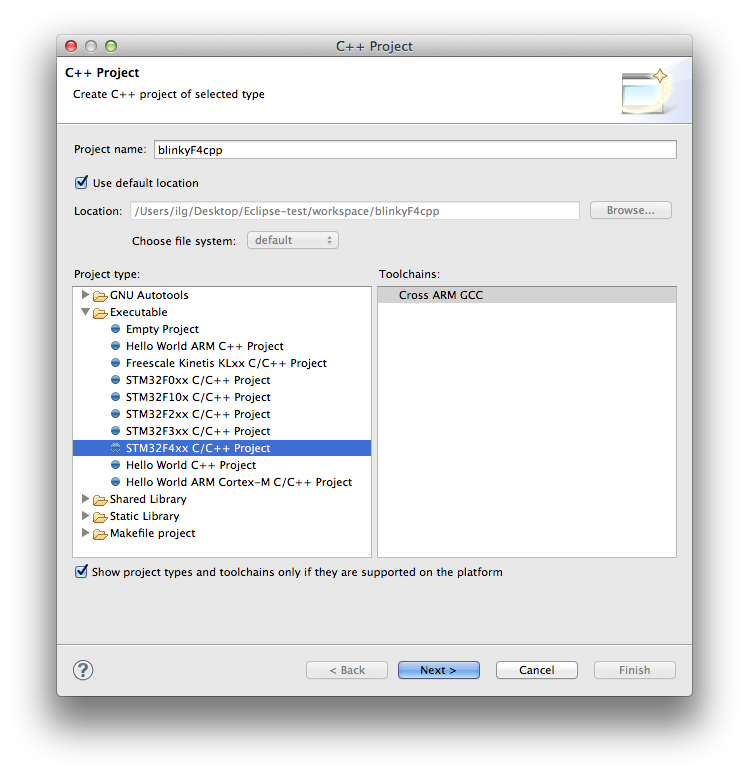
\includegraphics[width=0.4\textwidth]{Pictures/Einrichtung/NewF4Project.png}
	\caption{Erstellung eines Basisprojekts für den STM32F4 durch das GNU ARM Plugin. Ein Wizard Konfigurator führt den Anwender durch alle nötigen Einstellungen. Nach Abschluss erhält man ein fertiges C / C++ ARM Projekt welches passend zum Zielsystem konfiguriert ist.}
	\label{fig:NewProj}
\end{figure}
Das Templateprojekt beinhaltet bereits alle benötigten Hardware Bibliotheken (Abbildung \ref{fig:CMSIS}) wie den STM HAL (siehe Abschnitt \ref{sec:Zielsysteme}) oder das ARM CMSIS (Cortex Microcontroller Software Interface Standard).
\begin{figure}[htb]
	\centering
		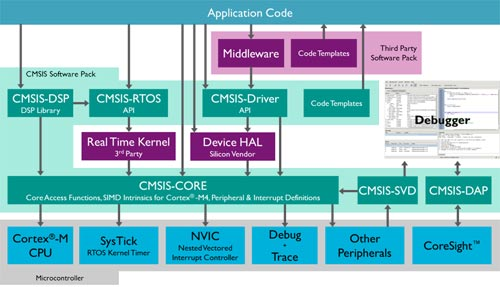
\includegraphics[width=0.4\textwidth]{Pictures/Einrichtung/CMSISv4_small.jpg}
	\caption{ARM embedded Anwendungen setzten auf unterschiedliche Abstraktionsschichten auf. Die untersten beiden Abstraktionsschichten sind CMSIS, welches Funktionen für ARM Devices bereitstellt, und der HAL des $\mu$Controller Herstellers. CMSIS steht für alle ARM Systeme zur Verfügung, wohingegen der HAL $\mu$Controller spezifisch ist. }
	%Ist HAL hier singular oder plural?
	\label{fig:CMSIS}
\end{figure}
Das Templateprojekt sollte jetzt kompilieren und mittels ISP-Programmer\footnote{In System Programmer} auf dem Zielsystem ausgeführt werden können.
Im nächsten Schritt wird FreeRTOS in das Templateprojekt eingebunden. Hierfür kann auf www.freertos.org die gepackte Variante der Demoprojekte heruntergeladen werden. Für den STM32F4 stehen spezielle Cortex M4 Portierungen zur Verfügung. Die Verzeichnisstruktur sollte dabei der Abbildung \ref{fig:SourceTree} ähneln.
\begin{figure}[htb]
	\centering
		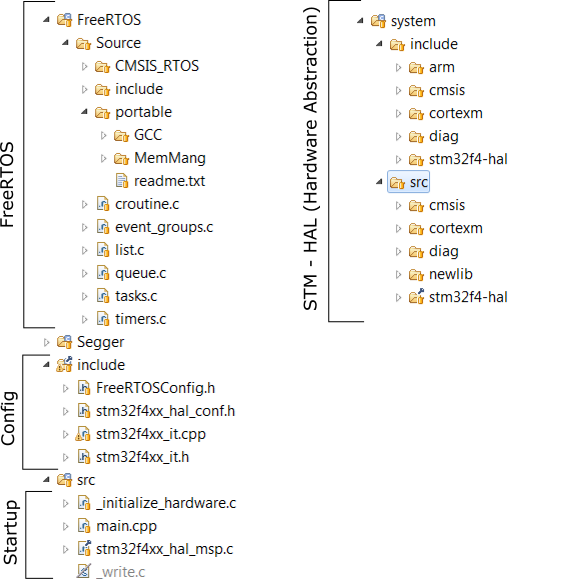
\includegraphics[width=0.4\textwidth]{Pictures/Einrichtung/sourceTree.png}
	\caption{Die Basiskonfiguration, die durch das GNU ARM Plugin zur Verfügung gestellt wird, besteht aus den Verzeichnissen: Startup, Config und HAL. Startup beinhaltet alle Files zum Starten der Hardware und die main-Funktion. Im Config Verzeichnis befinden sich alle Dateien zur Konfiguration des $\mu$Controllers und die FreeRTOS Config. HAL und CMSIS bilden die Grundlage des Systems und werden ebenfalls durch das GNU ARM Plugin eingefügt. FreeRTOS wird danach manuell dem Projekt hinzugefügt.}
	\label{fig:SourceTree}
\end{figure}
Nach der Anpassung der Include Pfade für den GCC Compiler und der Konfiguration der FreeRTOS Config ist die Einrichtung abgeschlossen.

%!TEX root = FreeRtos ARM uController.tex
%\pagebreak
\subsection{Memory Allocation}
Beim Erzeugen von RTOS Objekten wie Tasks, Queues oder Semaphore wird Speicher im RAM benötigt. Für die dynamische Speicherverwaltung wird in C und C++ ge\-wöhnlich die Standard C Funktionen malloc() und free() verwendet. Die Funktion malloc() dient zur Allozierung von freiem Speicher und free() zur Freigabe von alloziertem Speicher. Für Echtzeitsysteme, die auf einem RTOS aufsetzen, sind diese Funktionen aufgrund der folgende Eigenschaften\cite{MasteringFreeRtos} ungeeignet\footnote{Heap3 stellt hier eine Ausnahme dar}:
\needspace{3\baselineskip}
\begin{itemize}
	\item nicht thread safe
	\item nicht deterministisch
	\item tendieren zur Fragmentierung des RAM
	\item schwer zu debuggen
	\item Bibliotheksfunktionen benötigen viel Speicher
\end{itemize}
Des Weiteren sind für einige Einsatzgebiete von embedded Anwendungen Zertifikate erforderlich.\newline Speziell in sicherheitskritischen Anwendungen (Medical, Military) ist die dynamische Speicherverwaltung als eine potentielle Fehlerquelle auszuschließen. Für einen solchen Fall bietet FreeRTOS ab Version 9.0 die Möglichkeit der statischen Speicherallozierung, diese werden wir am Ende dieses Abschnitts betrachten. In FreeRTOS werden malloc() und free() durch die Funktionen  
\begin{lstlisting}[label=lst:vPortMalloc1, numbers = none]
void *pvPortMalloc( size_t xSize );
\end{lstlisting}
und
\begin{lstlisting}[label=lst:vPortFree1, numbers = none]
void vPortFree( void *pv );
\end{lstlisting}
ersetzt. Dies hat den Vorteil, dass die Implementierung dieser Funktionen an die jeweilige Anwendung angepasst werden kann. FreeRTOS stellt dem Entwickler fünf unterschiedliche Implementierungen von Speicheralgorithmen (Heap\_1.c bis Heap\_5.c) zur Verfügung, siehe Abbildung \ref{fig:HeapsEclipse}. 
\begin{figure}[htb]
	\centering
		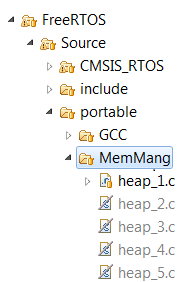
\includegraphics[width=0.2\textwidth]{Pictures/Eclipse/Heaps.png}
	\caption{Einbindung des Speicheralgorithmus Heap1 in Eclipse CDT. Die Algortihmen Heap2 bis Heap5 sind vom Build ausgeschlossen}
	\label{fig:HeapsEclipse}
\end{figure}
\begin{lstlisting}[caption={FreeRTOS Source von pvPortMalloc() aus Heap1.c. Zuerst wird sichergestellt das die Startspeicheradresse dem byte-Alignment des $\mu$\-Pro\-zesso\-rs entspricht. Der STM32F4 ist ein 32Bit $\mu$\-Pro\-zesso\-r und hat ein byte-Alignment von 4, so dass die Startadresse immer eine Potenz von 4 sein muss. Danach wird der Scheduler deaktiviert und geprüft ob genug Speicher zur Verfügung steht. Abschließend wird der Speicher im ucHeap reserviert.  }, linewidth=8cm,captionpos=b, label=lst:malloc2, float=htb]
void *pvPortMalloc( size_t xWantedSize )
{
void *pvReturn = NULL;
static uint8_t *pucAlignedHeap = NULL;
	#if( portBYTE_ALIGNMENT != 1 ){
		if( xWantedSize & portBYTE_ALIGNMENT_MASK )	{
			/* Byte alignment required. */
			xWantedSize += ( portBYTE_ALIGNMENT - ( xWantedSize & portBYTE_ALIGNMENT_MASK ) );
		}
	}
	#endif
	vTaskSuspendAll();
	if( pucAlignedHeap == NULL ){
		pucAlignedHeap = ( uint8_t * ) ( ( ( portPOINTER_SIZE_TYPE ) &ucHeap[ portBYTE_ALIGNMENT ] ) & ( ~( ( portPOINTER_SIZE_TYPE ) portBYTE_ALIGNMENT_MASK ) ) );
	}
	/* Check there is enough room left for the allocation. */
	if( ( ( xNextFreeByte + xWantedSize ) < configADJUSTED_HEAP_SIZE ) &&
		( ( xNextFreeByte + xWantedSize ) > xNextFreeByte )	)	{
		pvReturn = pucAlignedHeap + xNextFreeByte;
		xNextFreeByte += xWantedSize;
	}
	xTaskResumeAll();
	return pvReturn;
}
\end{lstlisting}
\begin{lstlisting}[caption={FreeRTOS Source von vPortFree() aus Heap1.c . Da eine Speicherfreigabe in Heap1 nicht vorgesehen ist, ist diese Funktion leer.}, linewidth=8cm,captionpos=b, label=lst:free2, float=htb]
void vPortFree( void *pv )
{
	/* Memory cannot be freed using this scheme. */
	( void ) pv;
	configASSERT( pv == NULL );
}
\end{lstlisting} 
Diese stellen prinzipiell schon die ge\-läu\-figsten Implementierungen zur Speicherverwaltung dar. Es bleibt aber auch weiterhin die Möglichkeit eine eigene Speicherverwaltung zu implementieren. In dieser Arbeit werden wir Heap1 etwas genauer betrachten um ein grund\-sätz\-liches Verständnis für die FreeRTOS Speicherverwaltung zu bekommen. Heap2 - Heap 5 werden nur kurz beschrieben und können im Detail in \cite{MasteringFreeRtos} und \cite{FreeRtosAdvanced} nachgelesen werden. Wie schon am Anfang dieses Abschnitts beschrieben, wird für alle RTOS Objekte Speicher benötigt. Der Speicher für Objekte wie Semaphore und Tasks wird automatisch in den statischen Erzeugerfunktionen der RTOS API alloziert, in dem intern die Funktion \textit{pvPortMalloc()} aufgerufen wird. Die Erzeugerfunktion xTaskCreate() beispielsweise, erzeugt eine FreeRTOS Task. Listing \ref{lst:xTaskCreate} zeigt wie xTaskCreate() die Funktion pvPortMalloc() verwendet um Speicher für den Stack und den Task Control Block zu allozieren.
\begin{lstlisting}[caption={FreeRTOS Source von xTaskCreate() aus Task.c. Jede Task bestitzt einen Stack und einen Task Control Block, beide werden beim Aufruf von xTaskCreate (Zeile 5 und Zeile 11) erstellt.}, linewidth=8cm,captionpos=b, label=lst:xTaskCreate, float=htb]
StackType_t *pxStack;
pxStack = ( StackType_t * ) pvPortMalloc(( ( ( size_t ) usStackDepth ) 
* sizeof( StackType_t ) ) );
if( pxStack != NULL )
{
	pxNewTCB = ( TCB_t * ) pvPortMalloc( sizeof( TCB_t ) );
	if( pxNewTCB != NULL )
	{
		pxNewTCB->pxStack = pxStack;
	}

}
\end{lstlisting}
Alle Objekte die mittels pvPortMalloc() alloziert werden, darunter auch der Kernel selbst, teilen sich einen gemeinsamen Adressraum, siehe Abbildung \ref{fig:AddressSpace}. 
\begin{figure}[hbt]
	\centering
		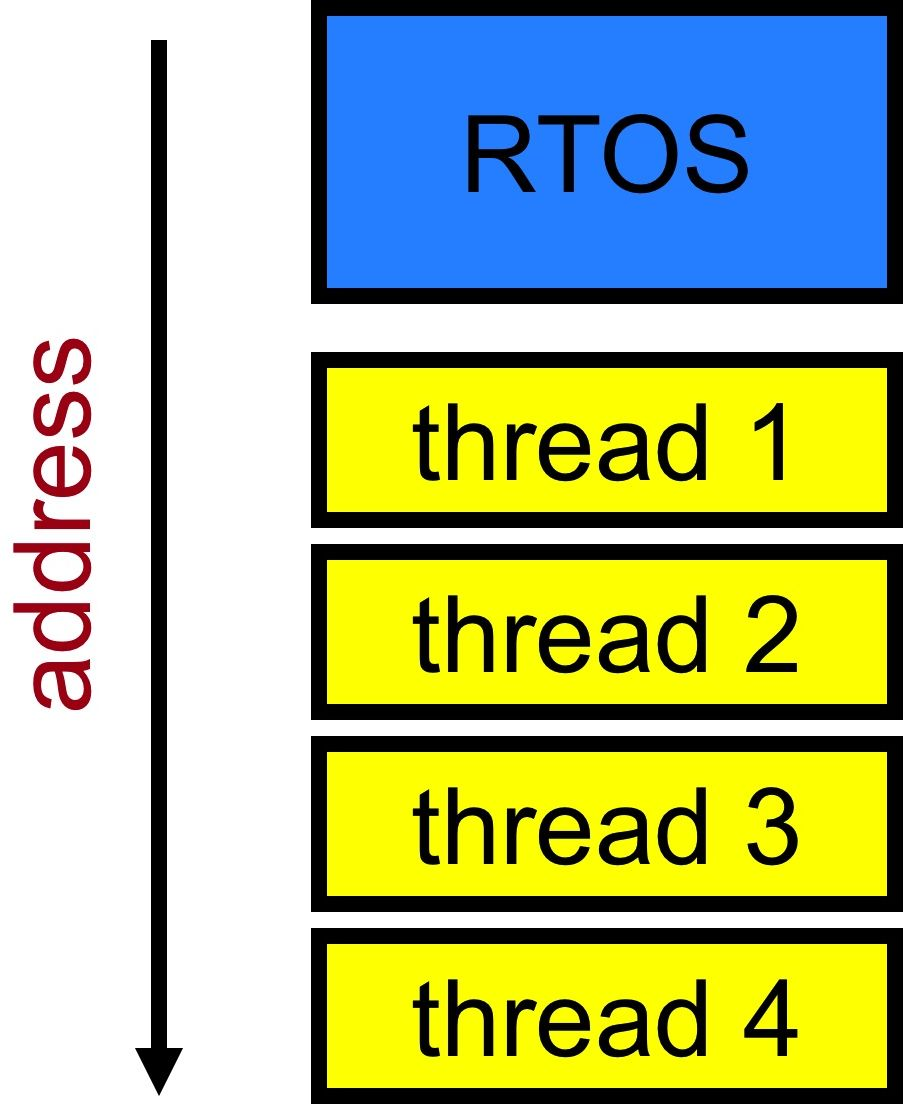
\includegraphics[width=0.2\textwidth]{Pictures/EmbeddedCom/addressSpace.jpg}
	\caption{Task und Kernel teilen sich in FreeRTOS einen gemeinsamen Adressraum. Dies stellt eine potentielle Fehlerquelle dar. Bild-Quelle~\protect\citeA{RTOSRevealed}}
	\label{fig:AddressSpace}
\end{figure} 
Durch den gemeinsamen Adressraum ist es möglich aus einer Task, auf die Variablen einer anderen Task zuzugreifen. Ein ungewollter Speicherzugriff ist somit durchaus möglich.\newline
In Abschnitt \ref{sec:Memory Protection} wird gezeigt welche Möglichkeit der STM32F4 und FreeRTOS bieten um Speicherzugriffe sicherer zu gestalten.    
\pagebreak 
%\cleardoublepage
%\FloatBarrier
\subsubsection{FreeRTOS Algorithmen zur Speicherverwaltung}
Bevor Objekte erzeugt werden können, muss ein Pool an Speicher für die Objekte definiert werden. Die einfachste Form einen Memory Pool zu erzeugen ist ein Array. In FreeRTOS nennt sich dieses Array ucHeap.
\begin{lstlisting}[numbers = none]
static uint8_t ucHeap[ configTOTAL_HEAP_SIZE ];
\end{lstlisting}
Die Größe des Heaps wird durch das Prä\-pro\-zes\-sor-Define configTOTAL\_HEAP\_SIZE (FreeRTOS\_config.h) konfiguriert. Die Gesamtgröße berechnet sich wie folgt:
\newline
\newline
MaxHeapSize $=$ configTOTAL\_HEAP\_SIZE $\ast$ Wortbreite\footnote{Beim STM32F4 ist die Wortbreite 32 bit} 
\newline
\newline
Die Speicherverwaltung durch Heap1 ist sehr einfach.\newline 
Heap1 deklariert lediglich die Funktion pvPortMalloc(). Die Funktion pvPortFree() wird nicht ausimplementiert. Abbildung \ref{fig:Heap1} zeigt wie der Speicher nach dem Erzeugen von zwei Tasks aussieht. 
\begin{figure}[htb]
	\centering
		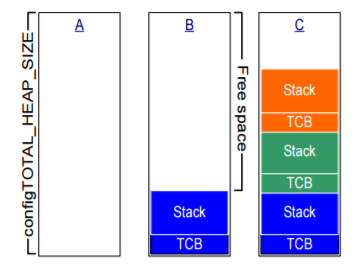
\includegraphics[width=0.3\textwidth]{Pictures/FreeRTOSOrg/heap1Alg.png}
	\caption{Beispiel Speicherbelegung nach drei Instanziierung von Tasks durch die Erzeugerfunktion xTaskCreate() unter Verwendung des Speicheralgorithmus Heap1. Bild-Quelle~\protect\citeA{MasteringFreeRtos}}
	\label{fig:Heap1}
\end{figure}
Für jede Task wird ein TCB und ein Stack erzeugt. Die Speicherobjekte liegen direkt hintereinander, da pvPortFree() nicht implementiert ist, kommt es auch nicht zu einer Fragmentierung des Speichers. Diese lineare Speicherzuweisung gilt für alle Objekte die mittels pvPortMalloc() alloziert werden, dazu gehören sowohl RTOS spezifische Objekte, als auch Objekte die durch den Entwickler erzeugt werden. Ein so einfacher Speicheralgorithmus wie Heap1 hat durchaus seine Berechtigung. Bei vielen embedded Anwendungen wird der Speicher für die benötigten Objekte vor dem Start des Schedulers erzeugt. Eine spätere Freigabe von belegten Ressourcen ist nicht nötig, da die Objekte über die gesamte Laufzeit des Programms bestehen sollen. Genau für solche Anwendungen steht Heap1 zur Verfügung. Nachfolgend ein Kurz\-über\-blick über die nicht beschriebenen Speicheralgorithmen.  
\begin{itemize}
	\item Heap2 - Ähnlich Heap1. Erlaubt allerdings Speicherfreigabe durch vPortFree(). Best Fit Algorithmus zur Speicherallozierung. 
	\item Heap3 - Verwendet C Library Malloc() und free() und deaktiviert den Scheduler zur Speicherallozierung.
	\item Heap4 - Ähnlicher Algorithmus wie bei Heap1 und Heap2. Verwendet First Fit Algorithmus zur Speicherallozierung. Verbindet mehrere kleinere Speicherblöcke zu einem Großen. Minimiert Speicherfragmentierung.
	\item Heap5 - Gleicher Algorithmus wie Heap4 allerdings kön\-nen mehrere Memory Pools erzeugt werden.
\end{itemize}
\subsubsection{Memory Protection}
\label{sec:Memory Protection}
Embedded Softwaresysteme können eine weitere Steigerung der Zuverlässigkeit erreichen, durch den Einsatz einer Memory Protection Unit (MPU). Die MPU bietet eine hardwarebasierende Lösung zur Detektion von ungewollten Speicherzugriffen (Abbildung \ref{fig:AddressSpaceMMU}). 
\begin{figure}[htb]
	\centering
		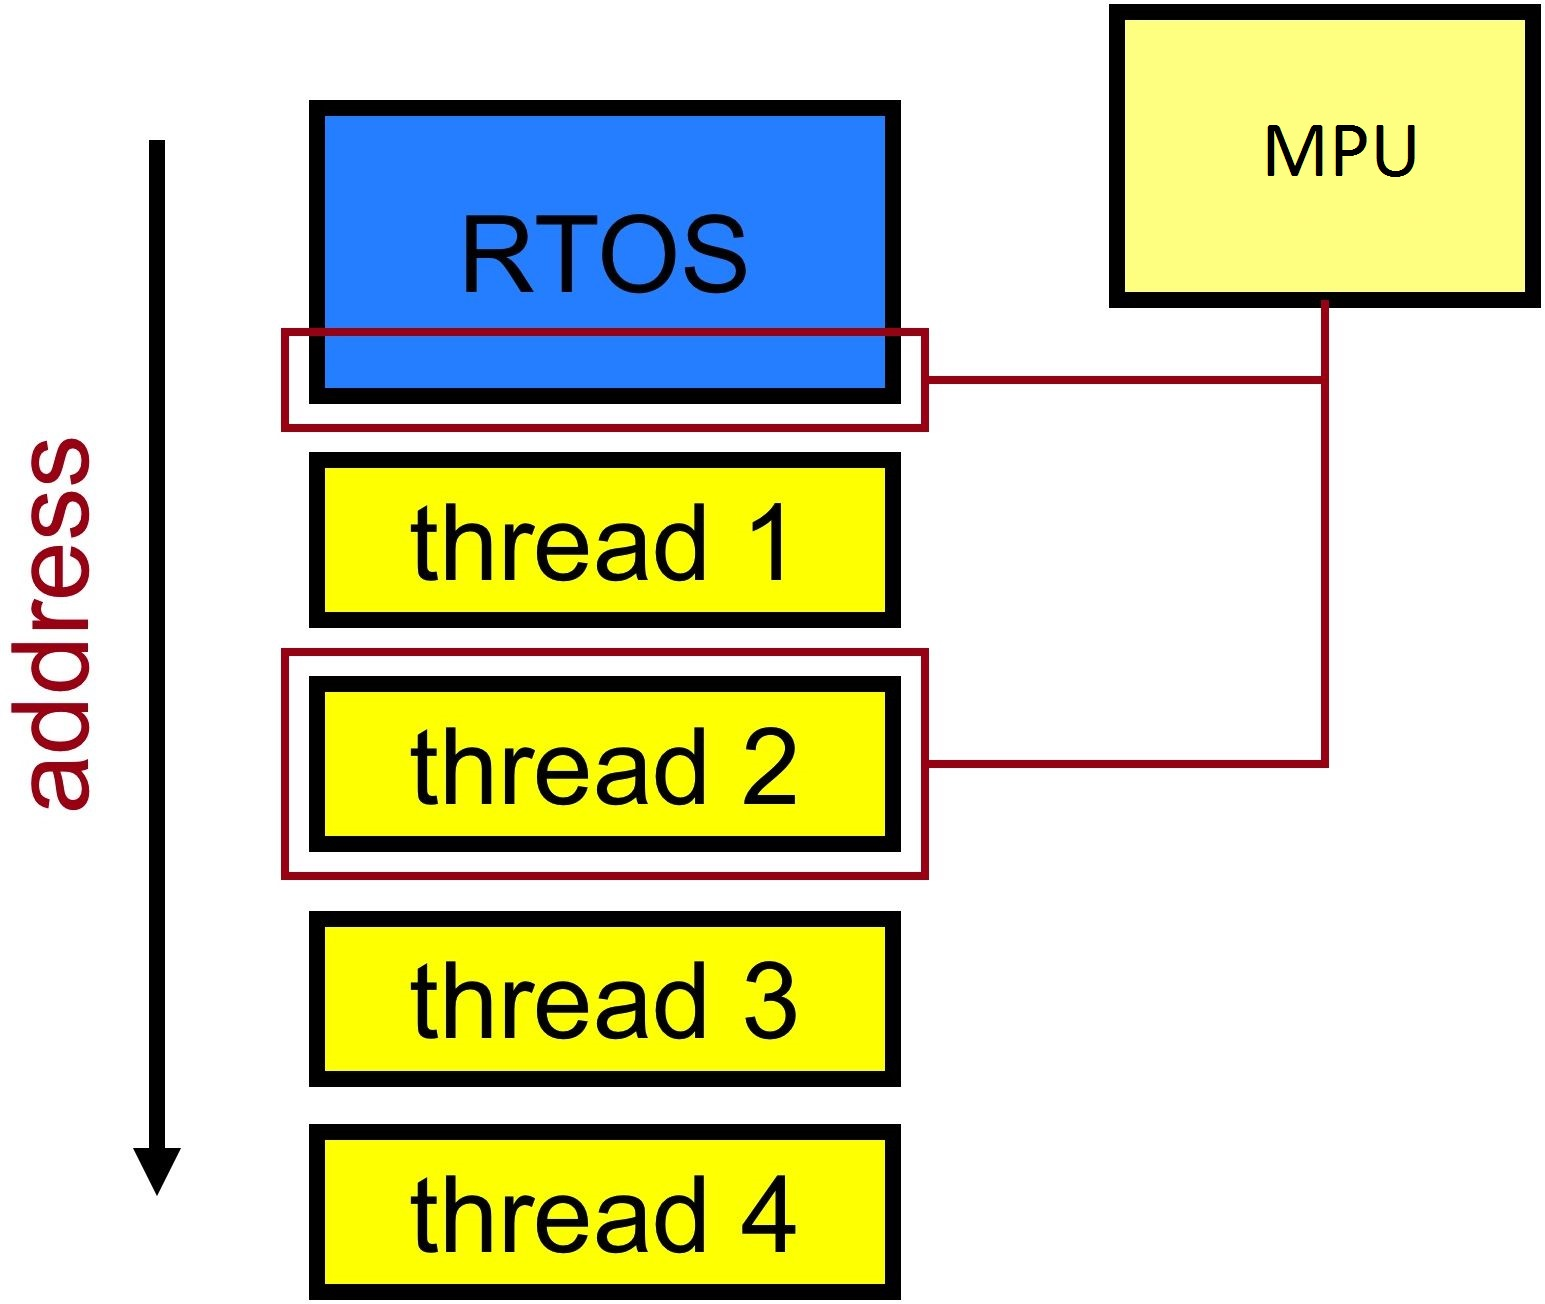
\includegraphics[width=0.3\textwidth]{Pictures/EmbeddedCom/addressSpaceMMU}
	\caption{Zugriffsrechte für Restricted Task wird durch den RTOS Kernel in der MPU konfiguriert. Der Speicherzugriff wir automatisch durch MPU/ MMU überprüft und im Fehlerfall an den Kernel gemeldet. Bild-Quelle~\protect\citeA{RTOSRevealed}}
	\label{fig:AddressSpaceMMU}
\end{figure} 
Für die MPU des STM32F4 $\mu$\-Pro\-zesso\-rs steht eine spezielle API Portierung von FreeRTOS zur Verfügung (FreeRTOS-MPU). Zur Erzeugung von Tasks, die die MPU nutzen sollen, muss die Erzeugerfunktion xTaskCreateRestricted() verwendet werden. Beim Aufruf der Erzeugerfunktion wird dem Kernel die Stackadresse der Task mitgeteilt, damit dieser die entsprechenden Zugriffsberechtigungen der Speicheradressen konfigurieren kann. Die so erzeugten Task werden Ristricted Task genannt. Der Zugriff aus einer Restricted Task auf den Speicher (Task-Stack) einer anderen Restricted Task, ist nicht erlaubt. Bei einem nicht erlaubten Speicherzugriff wird automatisch die entsprechende HookFunktion aufgerufen und ermöglicht es so dem System entsprechend zu reagieren. Restricted Task können sich in einem der folgenden Modis befinden:
\begin{itemize}
	\item User Mode
	\item Priviliged Mode 
\end{itemize}
Im User Mode ist es einer Restricted Task nicht erlaubt auf den Speicher des FreeRTOS Kernels zuzugreifen. So wird verhindert das der Kernel nicht ungewollt modifiziert wird. Nur einer Restricted Task, die sich im Priviliged Mode befindet, ist ein Zugriff auf den Kernel Speicher erlaubt. Dabei geschieht der Wechsel vom User Mode in den Priviliged Mode implizit durch den Aufruf einer FreeRTOS API Funktion. Ein Wechsel durch die Task selbst in den Priviliged Mode ist nicht möglich.
\subsubsection{Static Memory Allocation}
Die statische Speicherverwaltung wird durch das Prä\-pro\-zes\-sor-Define configSUPPORT\_STATIC\_ALLOCATION 1 in der FreeRTOS\_config aktiviert. Für die statische Objekterzeugung können die dynamischen Erzeugerfunktionen nicht mehr verwendet werden. Daher stehen spezielle Erzeugerfuntkionen für die statische Speicherallozierung zur Verfügung, wie xTaskCreateStatic() statt xTaskCreate() oder xSemaphoreCreateBinaryStatic() statt xSemaphoreCreateBinary(). Der Vorteil der statischen Speicherverwaltung ist, dass der belegte Speicher im RAM schon zur Übersetzungszeit bekannt ist und die potenzielle Fehlerquelle der dynamischen Speicherverwaltung vermieden\newline wird. Nachteil ist, dass mehr RAM verwendet wird als bei den meisten Heap Implementierungen. Heap1 stellt eine geeignete Alternative in der dynamischen Speicherverwaltung dar, da es die Risiken der dynamischen Speicherverwaltung auf ein Minimum reduziert.   

       
%!TEX root = FreeRtos ARM uController.tex
\subsection{Scheduling}
\label{Scheduling}
Der Scheduler ist die Kernkomponente jedes Echtzeitbetriebssystem Kernels, da er eine quasi parallele Ausführung von Tasks ermöglicht. Eine Task stellt dabei ein ei\-gen\-stän\-di\-ge lauffähige Programmeinheit dar und wird gewöhnlich in einer Schleife ausgeführt. Abhängig vom aktuellen Zustand der Tasks und dem gewählten Schedulingalgorithmus, wählt der Scheduler die nächste Task, die ausgeführt werden soll. Auf einem uProzessor mit einem Kern kann dabei immer nur eine Task zur Zeit ausgeführt werden. Der Vorgang des Task-Wechsels durch den Scheduler wird Kontextwechsel oder Kontextswitch genannt. Der Kontextwechsel ist für eine Task die verdrängt wird nicht erkennbar. Die Task wird bei ihrer aktuell ausgeführten Instruktion unterbrochen und alle nötigen Register under Stack werden durch den Scheduler gesichert. Abbildung \ref{fig:ContextSwitch} zeigt wie eine Task während ihrer Ausführung unterbrochen wird. Nachdem der Scheduler die verdrängte Task wieder zur Ausführung ausgewählt hat, werden alle Register und der Stack wieder hergestellt. Die Task wird danach ab der letzten Instruktion fortgeführt. 
\begin{figure}[ht!]
	\centering
		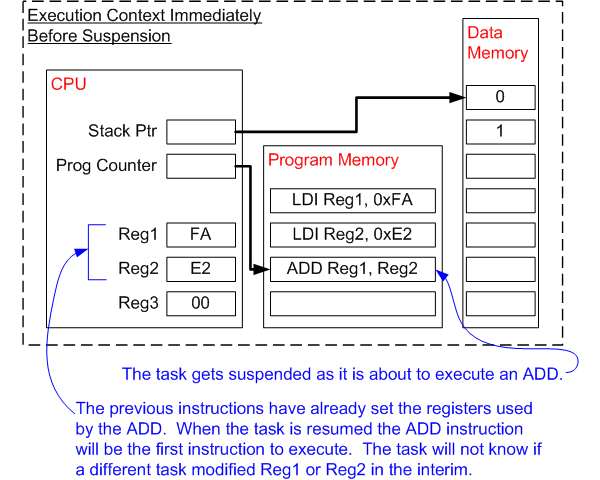
\includegraphics[width=0.4\textwidth]{Pictures/FreeRTOSOrg/ExeContext.png}
	\caption{FreeRTOS Pseudoimplementierung des Context - Switch. Bild-Quelle~\protect\citeA{MasteringFreeRtos} }
	\label{fig:ContextSwitch}
\end{figure}   
Folgende Zu\-stän\-de kann eine FreeRTOS Task annehmen: 
\begin{itemize}
	\item Running
	\item Blocked
	\item Ready
	\item Suspended
\end{itemize}
 Alle Tasks im Ready Zustand sind bereit und warten auf ihre Ausführung durch den Scheduler. Tasks die sich im Blocked Zustand befinden sind nicht bereit und warten auf ein Synchronisations- oder ein Timer Event. Eine Task die vTaskSuspend() aufruft, wird vom Scheduling Vorgang ausgeschlossen und nimmt den Zustand Suspended an. Abbildung \ref{fig:TaskStates} zeigt das Zustandsdiagramm einer FreeRTOS Task. 
\begin{figure}[ht!]
	\centering
		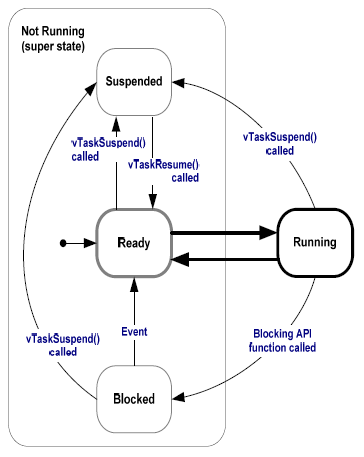
\includegraphics[width=0.3\textwidth]{Pictures/FreeRTOSOrg/taskStates.png}
	\caption{Übersicht aller Task Zustandstransitionen in FreeRTOS. Der Zustandswechsel findet entweder durch den Aufruf einer FreeRTOS API Funktion statt oder aber durch Event z.B. Interrupts, Timer-Events. Der Wechsel in den Zustand Running wird durch den Scheduler bestimmt und ist durch den Schedulingalgorithmus definiert.  Bild-Quelle~\protect\citeA{MasteringFreeRtos}}
	\label{fig:TaskStates}
\end{figure}Welche Task als näch\-stes vom Zustand Ready in den Zustand Running wechselt, wird durch den Scheduler bestimmt. Der Schedulingalgorithmus des Schedulers gibt dabei vor wie diese näch\-ste Task bestimmt wird. Der Scheduling Algorithmus des FreeRTOS Schedulers bietet unterschiedliche Kon\-fi\-gu\-ra\-tions\-mög\-lich\-kei\-ten auf die wir im laufe dieses Abschnittes genauer eingehen werden. Das Scheduling des FreeRTOS Kernels basiert grundsätzlich auf dem Round Robin Algorithmus\cite{9783827373427}. Dabei werden alle lauffähigen Tasks (Ready) gleicher Priorität in einer Liste verwaltet. Jede Task in der Liste erhält ein gewisses Zeitquantum\footnote{Round Robin definiert nicht die Länge des Zeitquantums}, welches bestimmt wie lange einer Task der Prozessor zugeteilt wird. Nach Ablauf des Zeitquantum wird ein Kontextwechsel durchgeführt und die näch\-ste Task in der Liste erhält Prozessorzeit. Die ausgelaufene Task wird durch den Scheduler automatisch hinten an die Liste angefügt. Jede Task in FreeRTOS wird eine gewisse Priorität zugewiesen, daher wird auch für jede Priorität eine eigene Round Robin-Liste geführt. Dieses Verfahren wird auch Priority Scheduling \cite{9783827373427} genannt. Abbildung \ref{fig:PrioList1} veranschaulicht das Ganze. In Listing \ref{lst:nextTask} wird gezeigt wie das Priority Scheduling im FreeRTOS Source Code umgesetzt wurde. 
\begin{figure}[ht!]
	\centering
		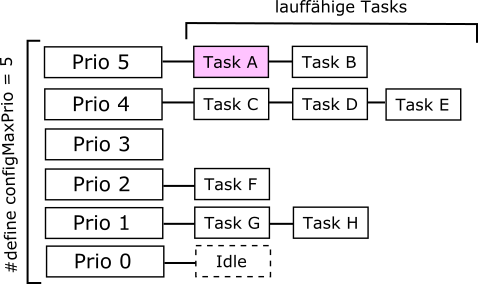
\includegraphics[width=0.3\textwidth]{Pictures/Scheduling/PrioList1.png}
	\caption{Aufbau der Prioritätenliste nach Round Robin in FreeRTOS. Alle aufgeführten Task sind bereit zur Ausführung. Task A wird aktuell durch den Scheduler ausgeführt. Nach dem Ablauf des Zeitquantums, wird A hinter B einsortiert. Die Maximale Priorität wird durch configMaxPrio bestimmt. Die Idle Task wird automatisch durch den Kernel erzeugt und hat immer die niedrigste Priorität. }
	\label{fig:PrioList1}
\end{figure}
\begin{lstlisting}[caption={FreeRTOS Source zur Priroty Task Selection aus Task.c. Alle lauffähigen Task werden in einem Array vewaltet pxReadyTaskLists. Die Listen verwalten sich durch Referenz-Pointer in den TCBs der einzelnen Tasks}, linewidth=8cm,captionpos=b, label=lst:nextTask, float=hbt]
#define taskSELECT_HIGHEST_PRIORITY_TASK(){																									
	UBaseType_t uxTopPriority = uxTopReadyPriority;														
		/* Find the highest priority queue that contains ready tasks. */								
		while(listLIST_IS_EMPTY(&(pxReadyTasksLists[ uxTopPriority ]))){																								
			configASSERT( uxTopPriority );																
			--uxTopPriority;																			
		}																								
		/* listGET_OWNER_OF_NEXT_ENTRY indexes through the list, so the tasks of						
		the	same priority get an equal share of the processor time. */									
		listGET_OWNER_OF_NEXT_ENTRY(pxCurrentTCB, &(pxReadyTasksLists[uxTopPriority]));			
		uxTopReadyPriority = uxTopPriority;																
	} /* taskSELECT_HIGHEST_PRIORITY_TASK */
\end{lstlisting}
Eine Besonderheit ist die Idle Task, diese wird automatisch beim Starten des Schedulers erzeugt. Die Idle Task hat die niedrigste Priorität und wird immer dann ausgeführt, wenn sich keine User-Task im Ready oder Running Zustand befindet. Die Idle Task ist ein Indikator für überschüssige Prozessorzeit. Mittels der Idle-Hook Funktion kann der Idle Task Funktionalität durch den Entwickler hinzugefügt werden. Wie die Idle Task zum Energiesparen genutzt werden kann, wird in Abschnitt \ref{sec:Low Power Modes} gezeigt. Wie bereits weiter oben beschrieben, lässt sich der Scheduling Algorithmus in verschiedenen Modis ausführen. Der Scheduler kann entweder im Cooperative Modus oder im Preemption Modus ausgeführt werden. Welcher Modus vom Scheduler verwendet wird, wird durch das define configUSE\_PREEMPTION in der FreeRTOS config bestimmt. Im Preemtive Modus wird eine aktive Task mit niedriger Priorität sofort von einer Task mit höherer Priorität verdrängt und ein Kontextwechsel wird durchgeführte. Im kooperativen Modus hingegen wird ein Kontextwechsel erst durchgeführt, wenn eine Task den Prozessor explizit durch die Funktion xTaskYield() abgibt. Abbildung \ref{fig:PreVSCo} zeigt den Vergleich beider Modis durch einen beispielhaften Ablauf. Eine weitere Option die sich über das define configUSE\_TIME\_SLICING aktivieren lässt ist das sogenannte Zeitschlitzverfahren. Durch das Zeitschlitzverfahren wird die zugeteilte Prozessorzeit für Task gleicher Priorität gleichmäßig aufgeteilt. Dies geschieht durch Einführung eines festen Tick-Interrupt Intervalls. Bei jedem Tick Interrupt wird der FreeRTOS SysTickHandler aufgerufen. Listing \ref{lst:SysTickS} zeigt die Implementierung des FreeRTOS SysTicks. Der SysTickHandler ist Bestandteil des Schedulers und überprüft bei jeder Ausführung, ob sich eine Task gleicher Priorität im Ready Zustand befindet. Sollte es eine solche Task geben wird ein Kontextwechsel durchgeführt und die Task erhält den Prozessor zugeteilt. Des Weiteren kümmert sich der SysTickHandler um die Verwaltung des TickCount, welcher als Referenz für alle RTOS Timingfunktionen dient. Abbildung \ref{fig:SysTick} zeigt diesen Vorgang nochmal im zeitlichen Verlauf. Die häufigst verwendete Scheduling Algorithmus nennt sich Prioritized Pre-emptive Scheduling with Time Slicing.
\begin{figure}[htb]
	\centering
		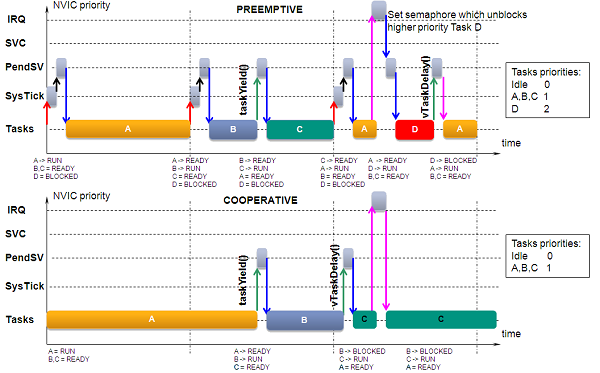
\includegraphics[width=0.5\textwidth]{Pictures/EMCUIT/PreemptiveCooperative.png}
	\caption{Im Co-operative Modus wird der Prozessor von einer Task erst abgegeben, wenn diese explizit taskYield() aufruft. Selbst wenn eine Task mit höhrer Priorität in den Ready Zustand wechselt, läuft die Task mit niedrigerer Priorität weiter. Im Gegensatz dazu steht das Pre-Emptive Scheduling (hier mit Time-Slicing), es unterbricht die laufende Task mit niedriger Priorität sofort, sobald eine Task mit höherer Priorität Ready ist. Bild-Quelle~\protect\citeA{MasteringFreeRtos}}
	\label{fig:PreVSCo}
\end{figure}
\begin{lstlisting}[caption={FreeRTOS Source des SysTickHandlers aus Task.c. Der SysTickHandler verwaltet den TickCount. Der TickCount dient allen Timingfunktionen des RTOS Kernels als Zeitreferenz. Des Weiteren wird bei aktivem Time Slicing überprüft ob ein Kontextwechsel nötig ist. Der Kontext wechsel wir dann ggf. durch den PendSVHandler durchgeführt.}, linewidth=8cm,captionpos=b, label=lst:SysTickS, float=hbt]
void xPortSysTickHandler( void ){
	/* The SysTick runs at the lowest interrupt priority, so when this interrupt
	executes all interrupts must be unmasked.  There is therefore no need to
	save and then restore the interrupt mask value as its value is already
	known. */
	portDISABLE_INTERRUPTS();
	{
		/* Increment the RTOS tick. */
		if( xTaskIncrementTick() != pdFALSE )
		{
			/* A context switch is required.  Context switching is performed in
			the PendSV interrupt.  Pend the PendSV interrupt. */
			portNVIC_INT_CTRL_REG = portNVIC_PENDSVSET_BIT;
		}
	}
	portENABLE_INTERRUPTS();
}
\end{lstlisting}
\begin{figure}[htb]
	\centering
		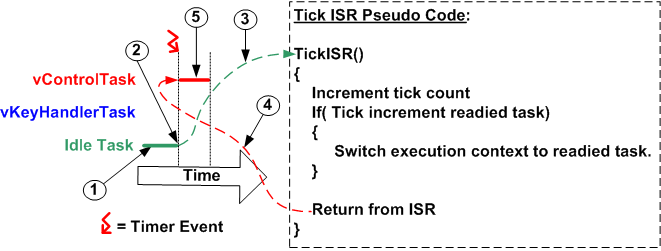
\includegraphics[width=0.4\textwidth]{Pictures/FreeRTOSOrg/TickISR.png}
	\caption{Beispielhafter Ablauf eines SysTickInterrupts.(1) keine User Task ist ready, die Idle Task ist aktiv. (2) SysTickInterrupt. (3) SysTickHandler wird aufgerufen. (4) vControlTask ist ready und ein Kontext wechsel wird durchgeführt. vControlTask hat hier die gleiche Priorität wie die IdleTask. (5)vControlTask wird ausgeführt. Bild-Quelle~\protect\citeA{MasteringFreeRtos}}
	\label{fig:SysTick}
\end{figure}


Listing \ref{lst:TaskExam1} zeigt ein minimal Beispiel einer Task und den Start des Schedulers durch vTaskStartScheduler() in der main function. 
\begin{lstlisting}[caption={Minimal Beispiel für die Definition eine Task. }, linewidth=8cm,captionpos=b, label=lst:TaskExam1, float=hbt]
 void main( void )
 {
	//Task werden oft vor dem Start des Schedulers erzeugt.
	xTaskCreate( vTaskCode,
							"NAME",
							STACK_SIZE,
							NULL,
							tskIDLE_PRIORITY,
							NULL );
   // Scheduler wird gestartet
   vTaskStartScheduler();
   // Hier sollten wir nicht hinkommen, da der Scheduler laeuft.
 }

void vTaskCode( void * pvParameters )
{
    for( ;; ){
        /* Task code wird hier Implementiert
				 z.B. warten auf eine Nachricht*/
    }
		/* Hier sollten wir nicht hinkommen*/
		vTaskDelete( NULL );
}
\end{lstlisting}


%!TEX root = FreeRtos ARM uController.tex
\subsection{Intertask Kommunikation}
Queues, Semaphore, Notify, Event Groups
In Projekten, in denen verschiedene Tasks parallel verarbeitet werden, ist es häufig erforderlich, dass diese Tasks die Möglichkeit besitzen Informationen untereinander auszutauschen. Sei es, weil ein Task Informationen produziert, die ein anderer Task für die weitere Verarbeitung benötigt, oder auch, weil beide Tasks gemeinsame Ressourcen (bspw. Hardwareregister) verwenden und sichergestellt werden muss, dass die dort hinterlegten Daten jederzeit korrekt sind. Wie bei normalen Betriebssystemen bietet auch FreeRTOS hier verschiedene Funktionen zur Interprozesskommunikation an. Zuerst sind hier die Queues zu nennen. Diese dienen dem klassischen Austausch von Informationen, indem Daten durch einen Task in die Queue hineingeschrieben werden und von einem zweiten Task gelesen werden. Meist bietet eine Queue die Option mehrere Datenpakete zu speichern. In FreeRTOS wird eine Queue mittels des Kommandos xQueueCreate(<uxQueueLength>,<uxItemSize>) angelegt.<uxQueueLength> bezeichnet hierbei die Anzahl der maximal speicherbaren Elemente, <uxItemSize> die Größe eines einzelnen Datums. Daten werden in FreeRTOS immer in eine Queue hineinkopiert. 
Es werden keine expliziten Queues angeboten die Pointer speichern. Es ist jedoch dennoch möglich Pointer als Datum in einer Queue zu hinterlegen, wodurch keine Einschränkung durch die fehlende Implementierung einer expliziten Zeigerqueue entsteht. Die Entwickler müssen hierbei jedoch sicherstellen, dass der Inhalt im Pointerziel immer konsistent ist und keine Speicherzugriffsverletzungen stattfinden.
Um einen Überlauf der Queue zu verhindern, werden Tasks die in eine Queue hineinschreiben wollen in den Zustand Blocked versetzt. Ebenso werden Tasks behandelt, die versuchen Daten aus einer leeren Queue abzurufen. Um die Echtzeitfähigkeit der Tasks weiter zu gewährleisten, bieten die Funktionen xQueueSendToFront(), xQueueSendToBack() und xQueueReceive() einen Parameter xTicksToWait an, mit dem festgelegt werden kann, wie lange eine Task maximal auf eine Antwort wartet. Erfolgt innerhalb dieser Zeit keine Antwort, so erhält die Task die Rückantwort errQUEUE_FULL bzw. errQueue_EMPTY und wird fortgesetzt. 
Sofern mehrere Tasks auf eine gemeinsame Queue zugreifen, so wird deren Zugriff im o.g. Fall zuerst nach Priorisierung der Task und danach durch Wartezeit gesteuert. Das heißt Zugriff auf die Queue zum Schreiben bzw. Lesen, je nach Zustand der Queue erhält die Task mit der höchsten Priorität. Existieren zwei Tasks mit der gleichen Priorität, so darf die Task zugreifen, die schon länger auf einen Zugriff wartet.
Zur Gruppierung von Queues werden Queue Sets angeboten, die mehrere verschiedenen Queues beinhalten. Die Entwickler von FreeRTOS empfehlen jedoch soweit möglich auf dieses Konstrukt zu verzichten. Daher sei es an dieser Stelle nur der Vollständigkeit halber erwähnt.
Neben Queues werden von FreeRTOS Mailboxes angeboten. Diese verhalten sich grundsätzlich wie Queues, beinhalten jedoch nur ein Datenobjekt, welches nach dem Lesen auch nicht direkt gelöscht wird, sondern in der Mailbox verbleibt, bis es von einer Daten erzeugenden Task überschrieben wird. Mailboxes sind vor allem in Szenarien interessant, in denen mehrere Tasks lesend auf ein erzeugtes Datum zugreifen sollen, beispielsweise eine Task zur Verarbeitung und eine niedriger priorisierte Task zur Anzeige.
//Semaphoren
FreeRTOS bietet Semaphoren für die Behandlung von Interrupts an. Hierbei werden zwei Formen der Semaphoren unterschieden. Zum Einen die Binären Semaphoren, die unter Umständen Interrupts verlieren können, zum Anderen die Counting Semaphoren, die die Interrupts mitzählen. Auf diesem Weg kann eine Task auch im Nachhinein feststellen, wie oft ein Interrupt ausgeführt wurde.
Die nächste Gruppe der Funktionen zur Interprozesskommunikation sind die Mutexes, eine Sonderform der Semaphoren. Semaphoren werden im folgenden Abschnitt behandelt. Mutexes werden benutzt um Zugriff auf gemeinsam genutzte Ressourcen zu steuern. Wenn ein Task auf eine Ressource zugreifen will, so prüft er vorher, ob er den Mutex erhalten kann. Ist dies nicht der Fall (weil ein anderer Task den Mutex besitzt) so muss der Task warten, bis der andere Task den Mutex zurück gibt. Zur Unterstützung von rekursiven Funktionen bietet FreeRTOS rekursive Mutexes an, die von einer Task mehrfach angefordert werden können.
Im Rahmen von Echtzeitsystemen müssen jedoch zwei Risiken beim Einsatz von Mutexes berücksichtigt werden. Zum einen können Deadlocks entstehen. Hierbei versuchen zwei (oder mehr) Tasks zeitgleich auf zwei (oder mehr) Ressourcen zuzugreifen. Beiden Tasks gelingt es mindestens einen Mutex zu erhalten. In der Folge kann keiner der Tasks vollen Zugriff auf die Ressourcen erlangen und wartet jeweils auf den anderen. Der Deadlock kann nur aufgebrochen werden, indem einer der Tasks seine Mutexes zurück gibt und der andere diese erhalten kann. Durch die notwendigen Timeouts kann die Echtzeitfähigkeit des Systems gefährdet werden.
Das andere Risiko besteht darin, dass eine niedrig priorisierte Task einen Mutex erhält und damit eine höher priorisierte Task von der Verwendung der Ressource ausschließt. FreeRTOS bietet hierzu eine Möglichkeit an, die niedrig priorisierte Task kurzzeitig auf die Priorität der hoch priorisierten Task zu setzen, sodass hier eine zeitnahe Abarbeitung stattfinden kann. Es kann jedoch auch hier zu Laufzeitproblemen kommen. Die Entwickler von FreeRTOS verwenden daher Wrapper-Funktionen, Gatekeeper genannt, die eine Kapselung der Ressourcen vornehmen und über Queues angesprochen werden. Auf diesem Weg kann auf den Einsatz von Mutexes weitestgehend verzichtet werden.
Die dritte und letzte Form der Intertaskkommunikation, die von FreeRTOS angeboten wird, ist die Task Notification. Sie ist die Variante mit dem geringsten Ressourcenaufwand, da anders als bei Queues und Mutexes keine Datenobjekte angelegt werden müssen. Durch das Aktivieren der Task Notifikation innerhalb der FreeRTOSConfig.h (Setzen von configUSE_TASK_NOTIFICATIONS auf 1) wird pro Task ein fester Speicherbereich reserviert, der für die Notification genutzt wird. Task Notifications werden direkt an die Zieltask gesendet. Es findet anders als bei Queues kein Zwischenspeichern der Information statt. Wenn eine Task eine andere Task benachrichtigt, so wird sie in den Zustand blockiert versetzt, bis der Notification Wert in den hierfür vorgesehen Speicherbereich geschrieben wurde. Darüber hinaus ist bei Notifications sichergestellt, dass die Informationen ausschließlich zwischen den beiden beteiligten Tasks ausgetauscht werden. Ein Zugriff eines dritten Tasks oder einer ISR (Interrupt Service Routine) auf diese Kommunikation ist ausgeschlossen.

%!TEX root = FreeRtos ARM uController.tex
\subsection{Interrupt Handling}
\label{sec:Interrupt}
%Michael: Notify hätte hier noch gut reingepasst, das es eine einfache, schnelle und leichtgewichtige Art ist um eine Task aus einer ISR zu informieren.
Interrupts können innerhalb von FreeRTOS auf verschiedenen Wegen behandelt werden. Hierbei bilden die Hardware gesteuerten Interrupt Service Routinen (ISR) die Basis. Um die Verarbeitungszeit für einen Interrupt kurz zu halten, führen ISRs gewöhnlich nur wenige Instruktionen aus. Dies geschieht beispielsweise durch das Informieren einer FreeRTOS Task mittels Intertaskkommunikation. Die FreeRTOS Task führt danach die eigentliche Aufgabe aus. Da die normalen API Funktionen für den Aufruf aus einen Task implementiert wurden und spezielle Eigenschaften eines Tasks verwenden, kann eine normale API Funktion nicht in einer ISR verwendet werden. Beispielsweise versetzen viele Intertask API Funktionen den aufrufenden Task in den Blocked Zustand. Dies ist im ISR Kontext natürlich nicht möglich. Damit man diese Funktionen dennoch nutzen kann, stellt FreeRTOS für die meisten API Funktionen spezielle ISR API Funktionen zur Verfügung. Diese Funktionen haben den postfix FromISR. ISR API Funktionen deaktivieren kurzfristig die Interruptverarbeitung innerhalb der kritischen Zugriffe.
FreeRTOS bietet verschiedene Mög\-lich\-keit\-en an, um Tasks einen Zugriff auf Interrupts zu ermöglichen.\newline
Zuerst die binären Semaphore, die mit xSemaphoreCreateBinary(void) erstellt werden. Hierbei handelt es sich um Speichervariablen, die einen binären Wert annehmen können. In dem Moment, in dem die Variable den Wert TRUE annimmt, ändert der Task seinen Zustand von Blocked auf Ready. Die Task kann in den Wartezustand gebracht werden, indem xSemaphoreTake() aufgerufen wird. Der Semaphor selbst wird durch eine ISR gesetzt. 
%Was meinst du damit ? Der Semaphor selbst wird durch eine ISR gesetzt. 
%Anpassen
Binäre Semaphore werden meist zu Synchronisationszwecken zwischen einem Task und einem Interrupt eingesetzt.
%Michael: Das wurde im Abschnitt vorher schon beschrieben. Wie gesagt eigentlich dient es zur synchroisierung von Zugriffen auf Ressourcen. 
Da nicht sichergestellt ist, dass die Task innerhalb der Zeitspanne, in der ein weiterer Interrupt auftreten kann, den vorhandenen Interrupt verarbeiteten kann, ist es möglich, dass ein Interrupt bei binären Semaphoren "'verloren'" geht.
%Michael: Das verstehe ich nicht, wie hilft hier ein Counting Semaphor, wenn man einen Interrupt verpasst? Ein counting Semphor würde sich doch auch verzählen. Ein counting semaphor wird doch für ressource genutzt die zählbar sind. z.B. es dürfen nur 5 Teilnehmer auf den Bus zugreifen. 
\newline Abhilfe schaffen hier die Counting Semaphore, die die nächste Zugriffsvariante auf Interrupts darstellen. Die Counting Semaphore werden durch das Setzen der folgenden Pre-Prozessor Direktive in der FreeRTOS Config aktiviert:
\begin{lstlisting}[numbers = none]
#define configUSE_COUNTING_SEMAPHORES  1
\end{lstlisting}
Im Anschluss kann die Semaphore mittels
\begin{lstlisting}[numbers = none]
xSemaphoreCreateCounting(uxMaxCount,uxInitialCount) 
\end{lstlisting}
angelegt werden. Die Counting Semaphore werden hierbei als Queue angelegt, die jedoch eher wie ein Zähler funktionieren. Der Parameter uxMaxCount legt hierbei fest, ab welchem Wert ein Überlauf des Zählers erfolgt. uxInitialCount legt den Wert des Zählers nach der Initialisierung fest. Im Anschluss können die Counting Semaphore wie binäre Semaphore verwendet werden. Der Aufruf von xSemaphoreTake() holt hierbei ein Semaphor-Objekt aus der Queue und versetzt den Task erst in den Blocked Zustand, wenn die Queue leer ist.
%Ggf. Kuerzen
Eine Möglichkeit um ganze Gruppen von Interrupts zusammenzufassen sind die Eventgroups. Hierbei geschieht die Tasksteuerung über Bitmasken. Innerhalb eines Tasks kann eine "`unblock condition"' definiert werden. Mit dieser kann definiert werden, ob der Task nur bei einer vollständig identischen Maske in den Zustand Ready wechselt, oder ob es bereits ausreicht, dass ein einzelnes Bit in der Maske gesetzt wird. Die Bedeutung der einzelnen Bits kann durch die Entwickler frei festgelegt werden. Eine Eventgroup wird mit dem Kommando xEventGroupCreate(void) erzeugt. Mittels xEventGroupSetBits(EventGroup,uxBitsToSet) werden die Bits uxBitsToSet innerhalb der Eventgroup gesetzt. Diese Funktion kann auch innerhalb von Tasks aufgerufen werden, beispielsweise zur Tasksynchronisation. Ein Task kann sich in den Blocked Zustand versetzen, indem xEventDroupWaitForBits() aufgerufen wird. Diese Funktion erhält außerdem als Parameter die Eventgroup, sowie die Bits, die beobachtet werden. Darüber hinaus wird mittels weiterer Parameter festgelegt, ob die aktuell gesetzten Bits zu\-rück\-ge\-setzt werden sollen.
%Michael: von Eventgroups wird laut RealTime Engineers abgeraten siehe : http://www.freertos.org/FreeRTOS-Event-Groups.html und Mastering FreeRTOS Kernal. Vielleicht bekommen die hier etwas viel Aufmerksamkeit :) 
%Als Quellen habe ich hier nur die Beschreibungen aus "`Mastering the FreeRTOS Kernel"' genommen
%!TEX root = FreeRtos ARM uController.tex
\subsection{Low Power Modes auf Stm32F4}
\label{sec:Low Power Modes}
Echtzeitbetriebssysteme kommen immer häufiger in akkubetriebenen embedded Systemen zum Einsatz. Solche Systeme verlangen eine effiziente Nutzung der Energieressourcen um einen möglichst langen Betrieb zu gewährleisten. Bezogen auf den uProzessor gibt es im Prinzip zwei Wege Energie einzusparen:
\begin{itemize}
	\item Heruntertakten des uProzessors.
	\item Das System schlafenlegen, wenn keine weiteren Aufgaben anstehen.
\end{itemize}
Das Heruntertakten des uProzessors ist unabhängig vom Einsatz eines RTOS, daher werden wir hier nur den zweiten Punkt genauer betrachten, das Schlafenlegen des uProzessors. 
\begin{figure}[htb!]
	\centering
		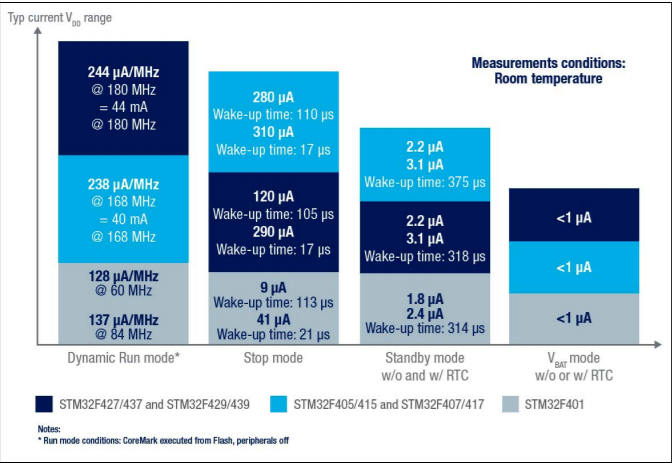
\includegraphics[width=0.4\textwidth]{Pictures/STM32F4/powerConsumption.png}
	\caption{Energieaufnahme für STM32F4 in SleepModes}
	\quelle{STM32F4 - Power Modes}
	\label{fig:powerconsum}
\end{figure}
Abbildung \ref{fig:powerconsum} zeigt wie sich die Stromaufnahme beim STM32F4 von 40mA im Normalbetrieb(@168 MHz) auf 2,2$\mu$A im Tiefschlafmodus reduzieren lässt. 
In einfachen Anwendung ist der Zustand in dem ein Gerät schlafen gehen kann, relativ leicht zu ermitteln. In komplexen Systemen die auf einem Echtzeitbetriebssystem wie FreeRTOS aufsetzen und mehrere Task mög\-li\-cherweise auf unterschiedliche Ressourcen warten, wird es schon schwierig. In diesem Abschnitt wird gezeigt welche Funktionen FreeRTOS zur Ver\-fü\-gung stellt, um einen energieeffizienten Betrieb zu gewährleisten. Eine Mög\-lich\-keit ist die Idle - Hook Funktion. Wie bereits in Abschnitt \ref{Scheduling} beschrieben, wird die IDLE Task von FreeRTOS aktiviert, sobald sich alle User-Tasks im Blocked Zustand befinden. Durch konfigurieren des Präprozessor-Defines        
\begin{lstlisting}[label=lst:defineIdleHook, numbers = none]
#define configUSE_IDLE_HOOK  1; 
\end{lstlisting}
\begin{lstlisting}[caption={Aufruf der IdleTask Hook Funktion. Aus Task.c},captionpos=b, label=lst:xIdleTaskHook, float=htb!]
static portTASK_FUNCTION( prvIdleTask, pvParameters )
{
	/* Stop warnings. */
	( void ) pvParameters;

	/** THIS IS THE RTOS IDLE TASK - WHICH IS CREATED AUTOMATICALLY WHEN THE
	SCHEDULER IS STARTED. **/

	for( ;; )	{
//skipped some code
#if ( configUSE_IDLE_HOOK == 1 )
{
	extern void vApplicationIdleHook( void );
	/* Call the user defined function from within the idle task.  This
	allows the application designer to add background functionality
	without the overhead of a separate task.
	NOTE: vApplicationIdleHook() MUST NOT, UNDER ANY CIRCUMSTANCES,
	CALL A FUNCTION THAT MIGHT BLOCK. */
	
	vApplicationIdleHook();
}
//guess what.. skipped more code
}     
\end{lstlisting}
kann die Idle-Hook Funktion aktiviert werden. Diese wird immer aufgerufen, sobald die Idle Task in den Zustand Running wechselt. Die Funktionalität der Idle-Hook Funktion kann frei vom Entwickler implementiert werden. Listing \ref{lst:xIdleHookExamp} zeigt Pseudocode zu einer beispielhaften Implementierung der Idle Hook Funktion. Bevor das System schlafen gelegt werden kann müssen alle GPIOS und IRQs konfiguriert werden, so dass das System nicht unnötiger weise aufwacht. Des Weiteren werden alle nicht benötigten GPIOS auf Analog gestellt um Energie zu sparen. Als einzige Interrupt-Quelle wird hier eine externe RTC konfiguriert. Mit dem Aufruf von HAL\_PWR\_EnterSTOPMode() wird der uProzessor in den Schlafmodus versetzt. Die Funktion wird erst wieder verlassen sobald der externe Interrupt der RTC ausgelöst wurde. Danach werden alle GPIOs rekonfiguriert. Ein weiterer Schritt der noch unternommen werden muss, ist das informieren einer User-Task z.B. mittels Notify oder Message, so dass das System nicht beim nächsten Tick Interrupt wieder die Idle Task aktiviert. Nachteil dieser Variante ist, dass die Nutzung von Software Timer nicht mehr möglich ist. Der FreeRTOS Kernel würde die Idle Hook Funktion auch aufrufen und sich schlafen legen, wenn noch Software Timer aktiv sind. Die Nutzung von absoluten Zeiten ist ebenfalls nicht mehr möglich, da nach der Deaktivierung des Tick Interrupts der Tickcount nicht mehr korrekt ist. Abhilfe schafft hier eine weitere Funktionalität die FreeRTOS zur Verfügung stell, den sogenannten Tickless Idle Mode. To be continued ....
\begin{lstlisting}[caption={Pseudocode für eine Idle Hook Funktion},captionpos=b, label=lst:xIdleHookExamp, float=hbt!]
extern "C" void vApplicationIdleHook( void ){
	/* Systick Interrupt deaktivieren */
	SysTick->CTRL &= ~SysTick_CTRL_TICKINT_Msk;
	//RTC konfigurieren
	setRTCWakeupTime();
	//externen Interrupt durch RTC aktivieren
	enableRTCInterrupt();
	//deaktiviere alle anderen Interrupt Quellen
	deactivateExternalDevices();
	setAllGPIOsToAnalog(); 
	disableGPIOClocks();
	//MCU stoppen und schlafen ZzZZz
	HAL_PWR_EnterSTOPMode(PWR_LOWPOWERREGULATOR_ON, PWR_STOPENTRY_WFI); 
	//Aufgewacht...the show must go on
	//aktiviere Systick
	SysTick->CTRL |= SysTick_CTRL_TICKINT_Msk;
	//reaktiviere GPIO Clocks
	enableGPIOClocks();
	//reaktiviere Externe Interrupt Quellen
	enableExternalInterrupts();	
}
\end{lstlisting}
\section{FreeRTOS in der Praxis} 
%!TEX root = FreeRtos ARM uController.tex
\subsection{Komplexität durch Nebenläufigkeit - Debugging von Echtzeitsystemen}
\label{sec:Debugging von Echtzeitsystemen}
TracerLyzer, RtosAwarenes, ThreadAwareness, Hardware Debugging Probes 
Probleme die bei der Entwicklung auftreten, Häufige Bugs, Speicherüberlauf (Stacktools)
\begin{figure}[ht!]
	\centering
		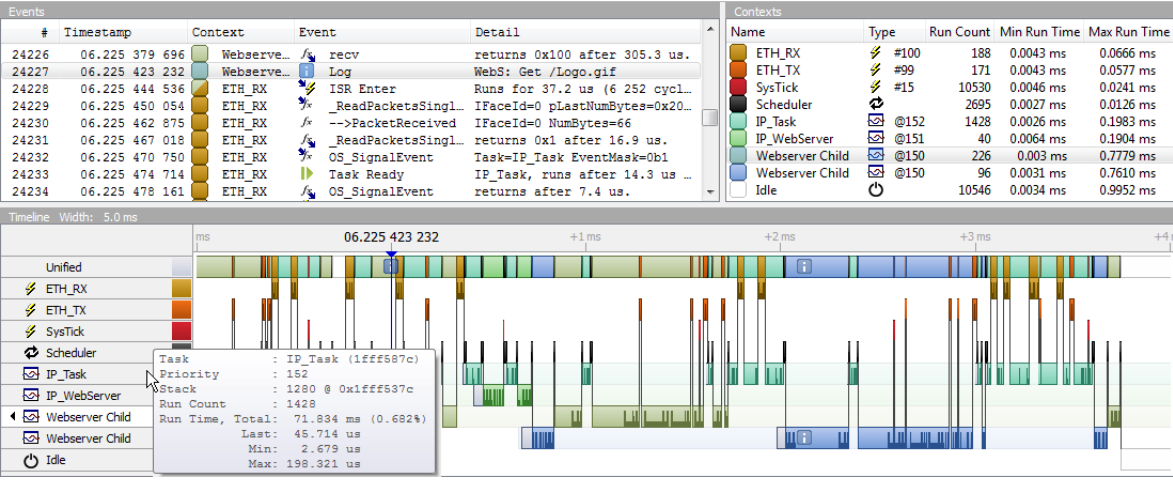
\includegraphics[width=0.5\textwidth]{Pictures/Segger/systemview.png}
	\caption{Segger Systemview - Not referenced yet}
	\label{fig:Systemview}
\end{figure}
\begin{figure}[ht!]
	\centering
		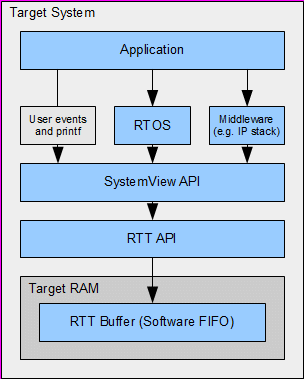
\includegraphics[width=0.3\textwidth]{Pictures/Segger/SystemViewTarget.png}
	\caption{Segger Systemview Target - Not referenced yet}
	\label{fig:SystemviewTarget}
\end{figure}
\begin{figure}[ht!]
	\centering
		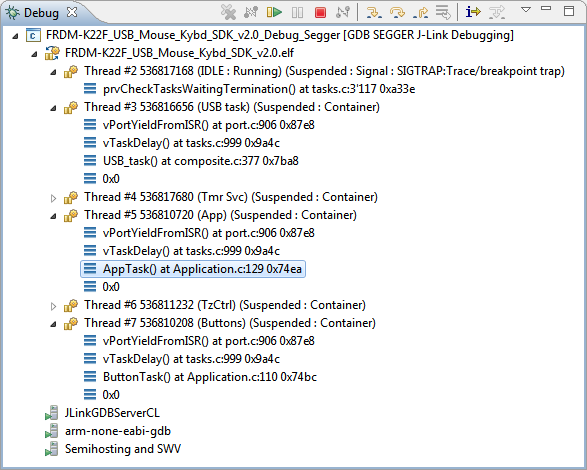
\includegraphics[width=0.5\textwidth]{Pictures/Segger/freertosThreadAwareness}
	\caption{Segger Thread Awareness- Not referenced yet}
	\label{fig:ThreadAware}
\end{figure}
%!TEX root = FreeRtos ARM uController.tex
\subsection{Echtzeitanalyse}
Uff :)
\label{sec:Echtzeitanalyse} 
%!TEX root = FreeRtos ARM uController.tex
\section{Zusammenfassung}
FreeRTOS kann als freies professionelles Echtzeitbetriebssystem betrachtet werden. Es ist steht den kommerziellen Echtzeitbetriebssystemen in Sachen Funktionalität in nichts nach. Bei den Herstellern von uControllern und ISP ist FreeRTOS eines des Standard Echtzeitbetriebssysteme. Es stehen gewöhnlich viele Beispiele oder Template Projekte für FreeRTOS zur Verfügung.  Besonders für Einsteiger ist FreeRTOS sehr zu empfehlen, da es kostenlos und sehr gut dokumentiert ist. Da FreeRTOS offenen Source Code zur Verfügung stellt, ist es dem Entwickler auch möglich einen Blick in die Implementierung des Echtzeitsystems zu werfen. Was besonders beim Verstehen des Kernels hilfreich ist. Da FreeRTOS auch in einer kommerziellen Version angeboten wird, kann davon ausgegangen werden, dass der Kernel auch langfristig Support erfährt. Ein Nachteil ist die komplizierte Einrichtung einer freien Entwicklungsumgebung wie Eclipse CDT, es bedarf enormen Konfigurationsaufwand bis eine Beispielanwendung mit FreeRTOS auf dem Zielsystem läuft.    
\pagebreak
\bibliographystyle{abbrv}
\bibliography{literatur} % Daten aus der Datei literatur.bib verwenden.
\end{document}

